\documentclass[journal]{IEEEtran}
\usepackage[utf8]{inputenc}
\usepackage[T1]{fontenc}
\usepackage{lmodern}
\usepackage[spanish,es-tabla]{babel}
\renewcommand{\IEEEkeywordsname}{Palabras clave}
\usepackage{booktabs}
\usepackage{makecell}
\usepackage{multirow}
\usepackage{float}
\usepackage{amsmath,amsfonts}
\usepackage{array}
\usepackage{url}
\usepackage{graphicx}
\usepackage{cite}
\setlength{\textfloatsep}{8pt plus 2pt minus 2pt}
\setlength{\floatsep}{5pt plus 2pt minus 2pt}
\setlength{\intextsep}{5pt plus 2pt minus 2pt}

\begin{document}

\title{Predicción de la Intención de Compra de Usuarios en Línea\\ mediante Aprendizaje Supervisado}

\author{Mateo Upegui Borja, Juan P. Uribe González, y Juan D. Rincón Bedoya%
	\thanks{Los autores son estudiantes de Ingeniería de Sistemas de la Universidad
		de Antioquia (UdeA), Medellín, Colombia.}
	\thanks{Este trabajo fue desarrollado para el curso de Modelos y Simulación II.}}

\markboth{Modelos y Simulación II, Universidad de Antioquia, Noviembre 2026}
{Entregable II: Predicción de la Intención de Compra}

\maketitle

\begin{abstract}
	Este documento integra el Entregable I corregido con las dos secciones del Entregable
	II: el diseño experimental y los resultados de cinco familias de modelos (30\,\%) y el
	análisis individual de variables con reducción de dimensión (20\,\%). Se usa el
	\textit{Online Shoppers Purchasing Intention Dataset} (UCI \#468), con 12\,330 sesiones,
	17 atributos predictores y una prevalencia de compra del 15,47\,\%. La tarea se formula
	como clasificación binaria supervisada de sesiones ya cerradas, no como predicción
	durante la sesión. El preprocesamiento y la selección de transformaciones se ajustan
	exclusivamente dentro de los folds de entrenamiento; el 20\,\% de validación se emplea
	para comparar finalistas y el 20\,\% de prueba se mantiene aislado. Se comparan regresión
	logística, k-NN, Random Forest, una red neuronal (MLP) y SVM con mallas ampliadas,
	intervalos de confianza bootstrap y comparaciones pareadas. Random Forest obtiene el
	mayor AP en prueba (0,7486) y la MLP el mayor ROC-AUC (0,9270); sin embargo, las
	diferencias pareadas entre ambos no son significativas (AP $+0{,}0104$,
	IC 95\,\% $[-0{,}0100;0{,}0321]$). La sensibilidad muestra que retirar
	\textit{PageValues} reduce el AP entre 0,34 y 0,39, mientras que retirar
	\textit{SpecialDay} no produce cambios apreciables. El umbral ajustado por F1 sube el
	recall de 0,466 a 0,717 en Random Forest. En la sección del 20\,\%, el análisis
	individual confirma el dominio de \textit{PageValues} (AUC 0,866); PCA retiene 28
	componentes y conserva el AP dentro de 1,7 puntos, mientras UMAP lo degrada entre 8 y
	16. Se discuten las implicaciones y limitaciones del alcance post-sesión.
\end{abstract}

\begin{IEEEkeywords}
	intención de compra, aprendizaje supervisado, clasificación binaria, validación
	cruzada, Random Forest, PageValues, PCA, UMAP.
\end{IEEEkeywords}

\section{Introducción}

El comercio electrónico genera un volumen alto de sesiones de navegación y solo una
fracción pequeña termina en compra. Identificar las sesiones con mayor probabilidad de
compra permite priorizar campañas de recuperación, segmentar visitantes y asignar
presupuesto de marketing con mejor criterio. El problema es relevante porque la señal
de compra es minoritaria y porque las decisiones de negocio suelen tener costos
distintos para los falsos positivos y los falsos negativos.

Este trabajo aborda la predicción de la intención de compra como un problema de
clasificación binaria supervisada sobre el \textit{Online Shoppers Purchasing Intention
Dataset} \cite{ref_dataset}. Cada observación es una sesión descrita por 17 atributos
de navegación, temporales y tecnológicos, y la etiqueta \textit{Revenue} indica si la
sesión terminó en compra. El objetivo es estimar, una vez cerrada la sesión, la
probabilidad de que haya terminado en compra, para segmentar y priorizar acciones
posteriores. No se promete una predicción durante la sesión: \textit{PageValues}, la
variable más informativa, se calcula con el resultado de la sesión y no está disponible
antes del cierre. El escenario sin \textit{PageValues} se analiza como prueba de
sensibilidad en la Sección~\ref{sec:sensibilidad}.

El trabajo tiene cinco aportes. Primero, define un protocolo reproducible en el que la
imputación, la transformación logarítmica, el escalado y la codificación se ajustan
dentro de cada fold, de modo que no hay fuga de información. Segundo, compara cinco
familias de modelos con mallas de hiperparámetros ampliadas y con una partición de
prueba que no participa en ninguna decisión. Tercero, reporta intervalos de confianza
bootstrap para AP, F1 y ROC-AUC, y comparaciones pareadas entre modelos, en lugar de
comparar solo medias puntuales. Cuarto, analiza el umbral de decisión y la sensibilidad
a \textit{PageValues} y \textit{SpecialDay}, dos variables que suelen discutirse sin
cuantificar su efecto. Quinto, evalúa cada variable por separado y compara PCA y UMAP
con la línea base para determinar si la señal se conserva al reducir la dimensionalidad.

El documento se organiza así. La Sección~\ref{sec:problema} describe el problema y el
paradigma. La Sección~\ref{sec:estado} revisa el estado del arte. La
Sección~\ref{sec:metodo} presenta los datos, el protocolo y las métricas. La
Sección~\ref{sec:resultados} reporta los resultados. La Sección~\ref{sec:reduccion}
analiza las variables y la reducción de dimensión. La Sección~\ref{sec:conclusiones}
discute las implicaciones y las limitaciones.

\section{Descripción del problema}
\label{sec:problema}

\subsection{Contexto y utilidad}

Una sesión de comercio electrónico reúne el rastro agregado de un visitante: páginas
consultadas, tiempo dedicado, tasas de rebote y salida, valor de las páginas visitadas,
cercanía a fechas especiales y características del dispositivo y de la fuente de
tráfico. La etiqueta \textit{Revenue} resume si la sesión terminó en compra. La
predicción post-sesión es útil para segmentar clientes, priorizar campañas de
recuperación y analizar qué perfiles convierten; también sirve como línea base para
estudiar un escenario operativo en el que la decisión deba tomarse antes del cierre,
pero ese escenario exige excluir las variables que se construyen con el resultado y
se trata aquí solo como sensibilidad.

La utilidad práctica depende del costo relativo de los errores. Un falso positivo
implica destinar una acción a una sesión que no comprará; un falso negativo implica
perder una compra que podría haberse recuperado. Por eso el informe reporta métricas
de ranking (AP y ROC-AUC), métricas de decisión (F1, precisión, recall y exactitud
balanceada) y el efecto de mover el umbral.

\subsection{Composición de los datos}

El conjunto contiene 12\,330 sesiones descritas por 18 columnas: 17 atributos
predictores y la etiqueta binaria \textit{Revenue}. La prevalencia de compra es del
15,47\,\% (1\,908 sesiones con compra frente a 10\,422 sin compra), lo que confirma un
desbalance marcado. La auditoría no encontró valores faltantes y sí 125 filas
duplicadas exactas. Esas 125 filas adicionales pertenecen a 201 filas agrupadas en
duplicados; todas son sesiones sin compra y todas tienen \textit{BounceRates} igual a
0,2. Es plausible que sean sesiones de rebote que coinciden en las 18 columnas. Se
eliminaron antes de particionar para evitar que una misma sesión apareciera en
entrenamiento y prueba. La decisión es conservadora: reduce el tamaño en 125 filas
(1,0\,\%) y no altera la clase positiva, que conserva sus 1\,908 casos.

Los atributos se agrupan en conteos de páginas administrativas, informativas y de
producto; duraciones de esas mismas categorías; tasas de rebote y salida; el valor de
página \textit{PageValues}; la cercanía a fechas especiales \textit{SpecialDay}; el mes
de la sesión; cuatro códigos enteros que representan categorías (sistema operativo,
navegador, región y fuente de tráfico); el tipo de visitante; y un indicador de fin de
semana. El conjunto contiene sesiones de diez meses: febrero, marzo, mayo, junio,
julio, agosto, septiembre, octubre, noviembre y diciembre. No hay sesiones de enero ni
de abril, de modo que el modelo no extrapola a esos meses; la cobertura mensual se
muestra en la Fig.~\ref{fig:datos}(b).

\textit{SpecialDay} toma seis valores equiespaciados (0; 0,2; 0,4; 0,6; 0,8; 1). Si se
codifica como ordinal $k=\mathrm{round}(\textit{SpecialDay}/0{,}2)$, la estandarización
de $k$ y la de \textit{SpecialDay} son transformaciones afines y producen la misma
matriz de diseño. Por eso el pipeline la trata como una variable numérica estandarizada
y la ablación de la Sección~\ref{sec:sensibilidad} confirma que retirarla no cambia el
AP de forma apreciable.

\subsection{Paradigma de aprendizaje}

Se elige aprendizaje supervisado porque la etiqueta está disponible y el objetivo es
predecir una clase conocida, no descubrir agrupamientos. La alternativa no supervisada
(clustering o reducción de dimensión) puede explorar perfiles, pero no sustituye la
predicción de \textit{Revenue}; se reserva para la sección de reducción de dimensión
del proyecto. Dentro del aprendizaje supervisado se comparan cinco familias que cubren
un espectro amplio de sesgo y varianza: un modelo lineal regularizado, un método
basado en vecinos, un ensamble de árboles, una red neuronal y una máquina de vectores
de soporte.

El desbalance aconseja no usar la exactitud como métrica principal. Un clasificador que
siempre prediga la clase mayoritaria supera el 84\,\% de exactitud y, sin embargo, no
detecta ninguna compra. Por eso la métrica principal es el área bajo la curva
precisión-recall (AP), que resume el compromiso entre precisión y recall en todos los
umbrales y es más informativa cuando la clase positiva es minoritaria. El ROC-AUC, el
F1 y la exactitud balanceada complementan el análisis. No se aplica sub ni
sobremuestreo en el experimento principal; se exploran pesos de clase balanceados
dentro de la validación cruzada, una alternativa que no genera datos sintéticos.

\section{Estado del arte}
\label{sec:estado}

La literatura que usa la misma base de datos permite situar los resultados. Cuatro
trabajos comparan familias de modelos con protocolos distintos
(Tabla~\ref{tab:estado}). Sakar \textit{et al.} \cite{ref_sakar} aplican sobremuestreo
y selección mRMR y reportan 87,24\,\% de exactitud y F1 0,86 con una MLP; Necula
\cite{ref_necula} combina K-means y PCA con ADASYN y obtiene un ROC-AUC de 0,9777 en
validación cruzada y 0,8973 en prueba con Random Forest; Satu e Islam \cite{ref_satu}
prueban SMOTE, tres escalados y filtros de variables y alcanzan 92,39\,\% de exactitud
y F1 0,924; Lin \cite{ref_lin} usa SMOTE, Isolation Forest y búsqueda de
hiperparámetros y reporta un ROC-AUC de 0,985 con CatBoost. Las cifras no son
comparables entre sí porque cambian la partición, el balanceo y el protocolo de
validación, y varios estudios no aclaran si el balanceo se ajusta solo con
entrenamiento. De ahí tres decisiones de este trabajo: ajustar todo el preprocesamiento
dentro de los folds, privilegiar AP, ROC-AUC y F1 frente a la exactitud, y cubrir la
ausencia de intervalos de confianza, comparaciones pareadas y análisis de umbral que se
observa en los antecedentes.

\begin{table*}[t]
\centering
\caption{Síntesis de los trabajos revisados con la misma base de datos.}
\label{tab:estado}
\scriptsize
\renewcommand{\arraystretch}{1.08}
\begin{tabular}{p{2.4cm} p{3.1cm} p{3.3cm} p{3.0cm} p{4.2cm}}
\toprule
\textbf{Trabajo} & \textbf{Modelos} & \textbf{Balanceo y selección} & \textbf{Validación} & \textbf{Métricas y resultado} \\
\midrule
Sakar \textit{et al.} \cite{ref_sakar} & MLP, RF, SVM & Sobremuestreo; correlación, información mutua y mRMR & 100 repeticiones de 70/30; prueba apartada antes del balanceo & MLP: exactitud 87,24\,\%, F1 0,86; con 6 variables mRMR: 87,94\,\% y 0,87 \\
Necula \cite{ref_necula} & LR, árboles, RF, SVM & ADASYN; análisis exploratorio con K-means y PCA & 10 folds estratificados; 25\,\% de prueba & RF: ROC-AUC 0,9777 en CV; en prueba 89,73\,\% y 0,8973. SVM: 90,21\,\% y 0,9021 \\
Satu e Islam \cite{ref_satu} & RF, SVM, árboles, LR & SMOTE, IQR, MinMax/Z-score/raíz; CFS, BFS, GRAE, IGAE & 10 folds en Weka & RF: 92,39\,\% de exactitud y F1 0,924; ROC-AUC 0,975 en otra configuración \\
Lin \cite{ref_lin} & SVM, XGBoost, CatBoost, red neuronal & SMOTE, Isolation Forest, selección por varianza, información mutua y correlación & 80/20 con 50 semillas; búsqueda en rejilla y aleatoria & CatBoost: precisión 0,934, recall 0,935, ROC-AUC 0,985. XGBoost: 0,935, 0,925 y 0,984 \\
\bottomrule
\end{tabular}
\end{table*}

La Tabla~\ref{tab:estado} confirma que las cifras no son directamente comparables:
cada estudio usa una partición, un balanceo y un protocolo distintos. Por eso este
trabajo ajusta el preprocesamiento dentro de los folds, aísla la prueba y reporta
incertidumbre; la comparación de las cinco familias y la verificación de
\textit{SpecialDay} retoman directamente las técnicas y advertencias de estos
antecedentes.

\section{Datos y configuración experimental}
\label{sec:metodo}

\subsection{Datos y codificación}

La Tabla~\ref{tab:variables} detalla el tipo, el significado y la codificación de cada
variable. Las variables numéricas (conteos, duraciones, tasas y \textit{PageValues}) se
imputan con la mediana, se transforman con $\log(1+x)$ si el hiperparámetro lo indica y
se estandarizan. La transformación $\log(1+x)$ admite ceros y reduce la asimetría de
las duraciones y de \textit{PageValues}; la decisión de usarla se selecciona por
validación cruzada, no se fija a priori. Las variables nominales
(\textit{Month}, \textit{OperatingSystems}, \textit{Browser}, \textit{Region},
\textit{TrafficType} y \textit{VisitorType}) se codifican con one-hot. Aunque
\textit{OperatingSystems}, \textit{Browser}, \textit{Region} y \textit{TrafficType} son
enteros, sus valores son códigos sin orden, de modo que tratarlos como números
introduciría una distancia artificial. \textit{Weekend} pasa directo como 0/1 y
\textit{SpecialDay} se estandariza. \textit{Revenue} es la etiqueta.

\begin{table*}[t]
\centering
\caption{Variables del conjunto, tipo, significado y codificación usada en el pipeline.}
\label{tab:variables}
\scriptsize
\renewcommand{\arraystretch}{1.05}
\begin{tabular}{p{3.0cm} p{2.1cm} p{7.0cm} p{4.2cm}}
\toprule
\textbf{Variable} & \textbf{Tipo} & \textbf{Significado} & \textbf{Codificación} \\
\midrule
\texttt{Administrative} & Conteo & Número de páginas administrativas visitadas & $\log(1+x)$ + estandarización \\
\texttt{Administrative\_Duration} & Continua (s) & Tiempo total en páginas administrativas & $\log(1+x)$ + estandarización \\
\texttt{Informational} & Conteo & Número de páginas informativas visitadas & $\log(1+x)$ + estandarización \\
\texttt{Informational\_Duration} & Continua (s) & Tiempo total en páginas informativas & $\log(1+x)$ + estandarización \\
\texttt{ProductRelated} & Conteo & Número de páginas de producto visitadas & $\log(1+x)$ + estandarización \\
\texttt{ProductRelated\_Duration} & Continua (s) & Tiempo total en páginas de producto & $\log(1+x)$ + estandarización \\
\texttt{BounceRates} & Continua & Tasa media de rebote de las páginas visitadas & $\log(1+x)$ + estandarización \\
\texttt{ExitRates} & Continua & Tasa media de salida de las páginas visitadas & $\log(1+x)$ + estandarización \\
\texttt{PageValues} & Continua & Valor medio de las páginas visitadas antes de la compra & $\log(1+x)$ + estandarización \\
\texttt{SpecialDay} & Ordinal (0--1) & Cercanía a una fecha especial (0 = lejos; 1 = mismo día) & Estandarización \\
\texttt{Month} & Nominal (10) & Mes de la sesión & One-hot \\
\texttt{OperatingSystems} & Nominal (código) & Sistema operativo del visitante & One-hot \\
\texttt{Browser} & Nominal (código) & Navegador del visitante & One-hot \\
\texttt{Region} & Nominal (código) & Región geográfica del visitante & One-hot \\
\texttt{TrafficType} & Nominal (código) & Fuente de tráfico de la sesión & One-hot \\
\texttt{VisitorType} & Nominal (3) & Tipo de visitante (nuevo, recurrente, otro) & One-hot \\
\texttt{Weekend} & Booleana & Indica si la sesión ocurrió en fin de semana & Pasa directo (0/1) \\
\texttt{Revenue} & Booleana (objetivo) & Indica si la sesión terminó en compra & Etiqueta \\
\bottomrule
\end{tabular}
\end{table*}

\begin{figure*}[t]
\centering
\begin{minipage}[t]{0.47\textwidth}
\centering
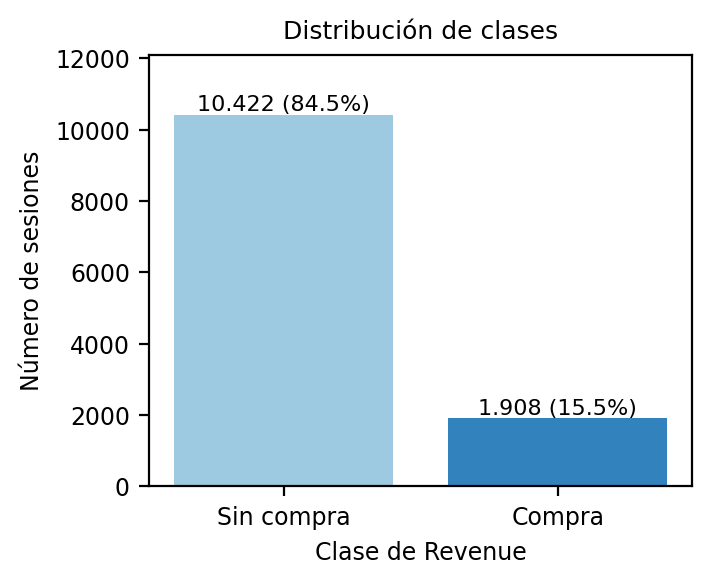
\includegraphics[width=\linewidth]{figuras/fig01_distribucion_clases.png}
\centerline{(a)}
\end{minipage}\hfill
\begin{minipage}[t]{0.51\textwidth}
\centering
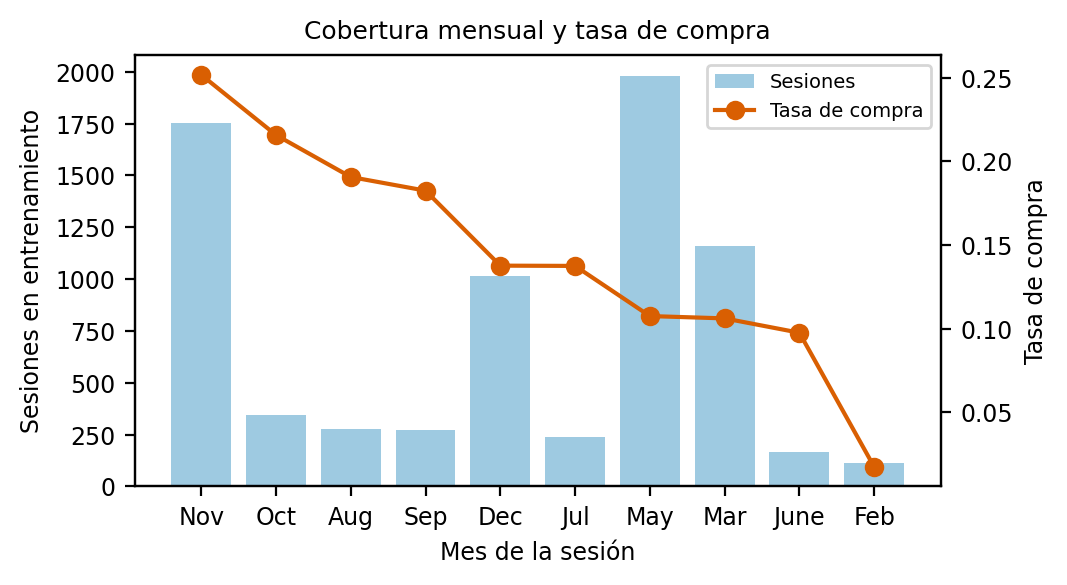
\includegraphics[width=\linewidth]{figuras/fig02_cobertura_mensual.png}
\centerline{(b)}
\end{minipage}
\caption{Exploración del conjunto. (a) Distribución de clases: 10\,422 sesiones sin
compra y 1\,908 con compra. (b) Cobertura mensual y tasa de compra en entrenamiento;
no hay sesiones de enero ni de abril.}
\label{fig:datos}
\end{figure*}

La Fig.~\ref{fig:datos}(a) muestra el desbalance y la Fig.~\ref{fig:datos}(b) la
cobertura mensual. Mayo concentra el mayor número de sesiones y noviembre la mayor
tasa de compra; la composición mensual no es uniforme, lo que refuerza la necesidad de
particiones estratificadas y de no extrapolar a los meses ausentes.

\subsection{Protocolo de validación}

Tras eliminar los duplicados exactos, el conjunto depurado se dividió de forma
estratificada en 60\,\% para entrenamiento, 20\,\% para validación y 20\,\% para prueba,
con semilla fija 42. La Tabla~\ref{tab:particiones} resume el tamaño y el balance. El
ajuste de hiperparámetros se realizó con validación cruzada estratificada de cinco
folds sobre el 60\,\% de entrenamiento, de modo que cada fold conserva la proporción de
compra. El 20\,\% de validación se empleó para comparar los finalistas y elegir el
ganador; el 20\,\% de prueba se mantuvo aislado hasta la evaluación final y no participó
en la selección de modelos, transformaciones ni hiperparámetros.

\begin{table}[t]
\centering
\caption{Tamaño y balance de las particiones tras eliminar duplicados exactos.}
\label{tab:particiones}
\footnotesize
\renewcommand{\arraystretch}{1.05}
\setlength{\tabcolsep}{3pt}
\begin{tabular}{lrrrr}
\toprule
\textbf{Partición} & \textbf{n} & \textbf{Compra} & \textbf{No compra} & \textbf{Prop.} \\
\midrule
Entrenamiento & 7\,323 & 1\,145 & 6\,178 & 15,64\,\% \\
Validación & 2\,441 & 381 & 2\,060 & 15,61\,\% \\
Prueba & 2\,441 & 382 & 2\,059 & 15,65\,\% \\
\midrule
Total & 12\,205 & 1\,908 & 10\,297 & 15,63\,\% \\
\bottomrule
\end{tabular}
\end{table}

Todo el preprocesamiento se encapsuló en un \texttt{Pipeline} y un
\texttt{ColumnTransformer}: la imputación, la transformación logarítmica, el escalado
y la codificación se aprenden únicamente con los datos de entrenamiento de cada fold.
No se aplicó sub ni sobremuestreo en el experimento principal. Se exploraron pesos de
clase balanceados como hiperparámetro, una alternativa que no genera datos sintéticos y
que se ajusta dentro de cada fold. El código, las particiones y los resultados se
conservan en el repositorio del proyecto; el entorno usado fue Python 3.13.5,
scikit-learn 1.7.2, pandas 2.3.1 y Matplotlib 3.10.7.

\subsection{Hiperparámetros y mallas}

La Tabla~\ref{tab:mallas} resume las mallas. Se ampliaron los rangos de los
hiperparámetros que en una primera exploración quedaban en el borde: $k$ de k-NN,
$C$ y $\gamma$ de SVM, y la tasa de aprendizaje y la arquitectura de la MLP. La malla
de SVM se separó en dos búsquedas, una para el kernel lineal y otra para el RBF, porque
$\gamma$ solo aplica al RBF; así se evitan combinaciones duplicadas. En total se
evaluaron 268 combinaciones efectivas: 20 de regresión logística, 56 de k-NN, 64 de
Random Forest, 48 de MLP y 80 de SVM (20 lineales y 60 RBF).

\begin{table*}[t]
\centering
\caption{Mallas de hiperparámetros y parámetros fijos.}
\label{tab:mallas}
\scriptsize
\renewcommand{\arraystretch}{1.08}
\begin{tabular}{p{2.6cm} p{4.8cm} p{8.0cm}}
\toprule
\textbf{Modelo} & \textbf{Hiperparámetros explorados} & \textbf{Parámetros fijos y número de combinaciones} \\
\midrule
Regresión logística & $C\in\{0{,}01;0{,}1;1;10;100\}$; \textit{class\_weight} $\in\{\text{ninguno},\text{balanced}\}$; $\log(1+x)\in\{\text{sí},\text{no}\}$ & \textit{solver}=lbfgs, \textit{max\_iter}=3000; 20 combinaciones \\
k-NN & $k\in\{5;15;31;45;61;81;101\}$; \textit{weights} $\in\{\text{uniform},\text{distance}\}$; $p\in\{1;2\}$; $\log(1+x)\in\{\text{sí},\text{no}\}$ & 56 combinaciones \\
Random Forest & \textit{max\_depth} $\in\{\text{sin límite};12;20;30\}$; \textit{min\_samples\_leaf} $\in\{1;5\}$; \textit{max\_features} $\in\{\text{sqrt};0{,}5\}$; \textit{class\_weight} $\in\{\text{ninguno},\text{balanced}\}$; $\log(1+x)\in\{\text{sí},\text{no}\}$ & \textit{n\_estimators}=300; 64 combinaciones \\
MLP & capas ocultas $\in\{(32,);(64,);(64,32)\}$; $\alpha\in\{0{,}0001;0{,}01\}$; \textit{learning\_rate\_init} $\in\{0{,}001;0{,}01;0{,}03;0{,}1\}$; $\log(1+x)\in\{\text{sí},\text{no}\}$ & \textit{solver}=adam, \textit{max\_iter}=500, \textit{early\_stopping}=True, \textit{validation\_fraction}=0{,}15, \textit{n\_iter\_no\_change}=20; 48 combinaciones \\
SVM & \textit{kernel} $\in\{\text{lineal},\text{RBF}\}$; $C\in\{0{,}1;1;10;30;100\}$; $\gamma\in\{\text{scale};0{,}01;0{,}001\}$ (solo RBF); \textit{class\_weight} $\in\{\text{ninguno},\text{balanced}\}$; $\log(1+x)\in\{\text{sí},\text{no}\}$ & 20 lineales + 60 RBF = 80 combinaciones \\
\bottomrule
\end{tabular}
\end{table*}

La ampliación de la malla de la MLP produjo un óptimo de validación cruzada en
$(64,32)$ con \textit{learning\_rate\_init}=0,1 (AP 0,7343). Sin embargo, al evaluar
esa configuración en el 20\,\% de validación, su AP fue 0,6939, inferior al 0,7134 de
la configuración $(64)$ con tasa 0,01. Como el conjunto de validación es el que decide
entre finalistas, se conservó la configuración $(64)$ con tasa 0,01 y se reporta la
ampliación como análisis de robustez. Este resultado ilustra que la selección por
validación cruzada no es inmune a la variabilidad entre folds y que conviene contrastar
los finalistas en una partición independiente.

Para descartar que 0,1 fuera un nuevo borde, se probaron tasas de 0,3 y 1,0 con el
resto de la malla fijo; ninguna superó el AP de validación cruzada de 0,1, de modo que
el óptimo de la tasa quedó en el interior del rango explorado.

\subsection{Métricas e intervalos de confianza}

La métrica principal es el área bajo la curva precisión-recall (AP), calculada como el
promedio de la precisión en los distintos umbrales de recall. Se complementa con el
ROC-AUC, que mide la capacidad de ordenar las sesiones por probabilidad de compra; con
el F1, la precisión y el recall de la clase positiva; y con la exactitud balanceada,
que promedia el desempeño en ambas clases. El punto de referencia trivial, que siempre
predice la clase mayoritaria, obtiene un AP igual a la prevalencia (0,156) y una
exactitud del 84,4\,\%.

Todas las medidas se reportan con intervalos de confianza del 95\,\% estimados mediante
bootstrap estratificado con 2\,000 réplicas, en entrenamiento, validación y prueba.
Además de los intervalos por modelo, se realizaron comparaciones pareadas en prueba:
para cada réplica se remuestrean por separado las clases positiva y negativa, se
calculan las métricas de los dos modelos sobre la misma réplica y se registra la
diferencia. Este diseño reduce la varianza de la comparación y permite afirmar si dos
modelos se distinguen más allá de la variabilidad del muestreo.

\section{Resultados}
\label{sec:resultados}

\subsection{Efecto de los hiperparámetros}

La Fig.~\ref{fig:hiperparametros} muestra el AP medio de validación cruzada para cada
valor de los hiperparámetros principales. Cada punto promedia el AP sobre las demás
combinaciones de la malla; la línea de entrenamiento es el promedio correspondiente.
La configuración ganadora de cada familia se reporta en la Tabla~\ref{tab:mejores}.

\begin{figure*}[t]
\centering
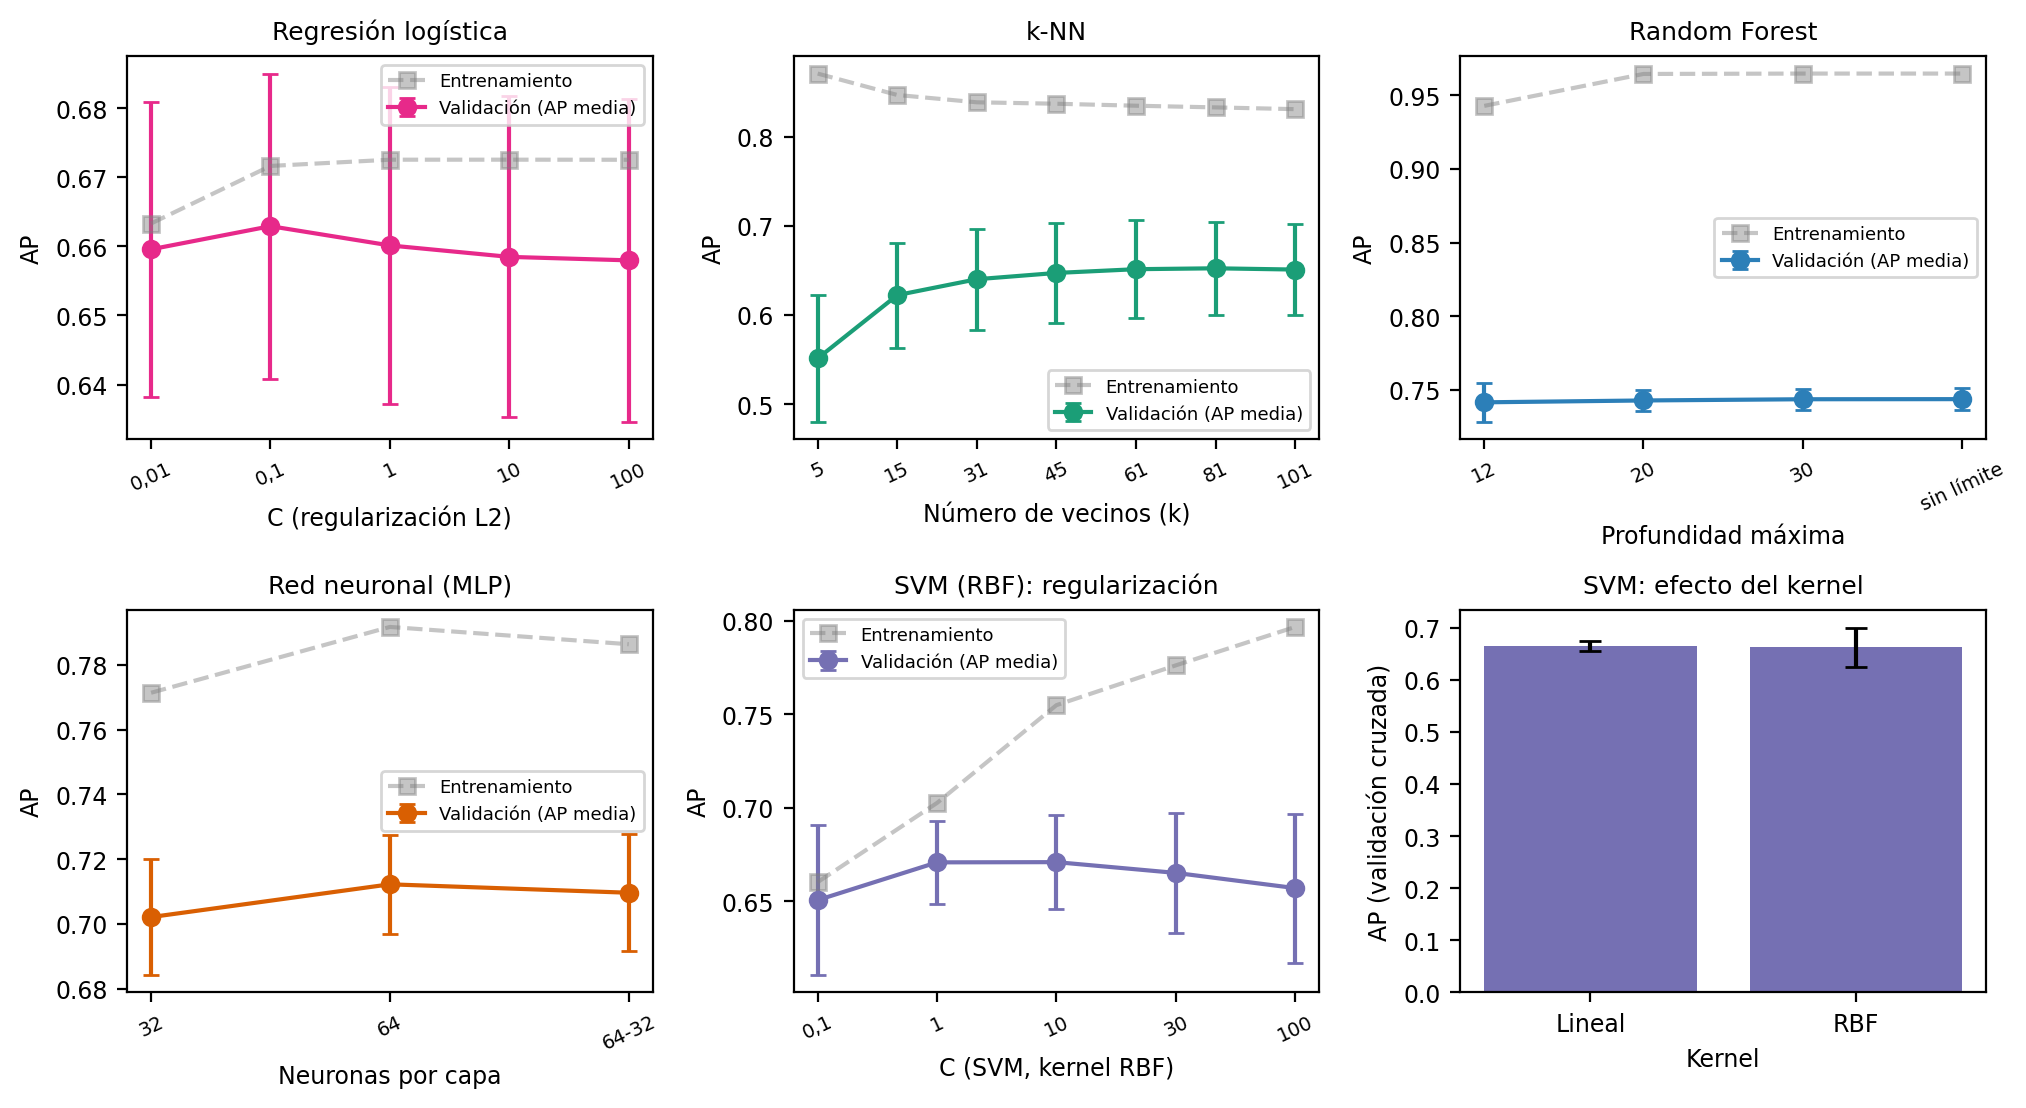
\includegraphics[width=\textwidth]{figuras/fig03_efecto_hiperparametros.png}
\caption{AP de validación cruzada frente a los hiperparámetros principales. Cada punto
es el promedio marginal sobre las demás combinaciones de la malla; las barras son la
desviación entre folds. La línea gris es el AP de entrenamiento. En Random Forest,
``sin límite'' corresponde a \textit{max\_depth}=None.}
\label{fig:hiperparametros}
\end{figure*}

En Random Forest, la profundidad tiene un efecto pequeño: 12 niveles dan un AP medio de
0,7414, 20 dan 0,7427, 30 dan 0,7435 y sin límite 0,7436. Las diferencias son menores
que la desviación entre folds (0,007--0,013), de modo que no hay evidencia de que una
profundidad mayor mejore el AP marginal. La mejor combinación conjunta, sin embargo,
usa 12 niveles (Tabla~\ref{tab:mejores}); la diferencia con las alternativas es
pequeña y debe leerse como una zona plana, no como una ventaja fuerte.

En SVM, el promedio marginal del kernel lineal (0,6648) es ligeramente superior al del
RBF (0,6623), pero la mejor configuración RBF (0,7266) supera con claridad a la mejor
lineal (0,6816). La aparente contradicción se explica porque la malla RBF incluye
combinaciones de $C$ y $\gamma$ con desempeño bajo que arrastran el promedio. Para el
kernel RBF, $C=1$ y $C=10$ son los mejores valores (0,6729 y 0,6731), mientras que
$C=0{,}1$ es el peor (0,6454); $C=10$ y $\gamma=0{,}01$ es la configuración ganadora.

En regresión logística, $C=0{,}1$ obtiene el mayor AP marginal (0,6629), seguido de
$C=1$ (0,6601); los extremos $C=0{,}01$ y $C=100$ quedan por debajo. En k-NN, el AP
marginal crece con $k$ hasta estabilizarse alrededor de 61--101: 0,6512 en $k=61$,
0,6522 en $k=81$ y 0,6508 en $k=101$. La mejor combinación conjunta usa $k=61$ con
\textit{weights}=distance y $p=2$ (AP 0,7203), lo que confirma que el óptimo quedó en
el interior de la malla ampliada. En la MLP, las arquitecturas $(64)$ y $(64,32)$ son
similares en promedio (0,7122 y 0,7096) y la tasa 0,01 es la mejor en promedio
(0,7119); la interacción con $\alpha$ y la arquitectura explica que la mejor
combinación conjunta use $(64,32)$ con tasa 0,1, como se discutió en la
Sección~\ref{sec:metodo}.

El AP de entrenamiento confirma el sobreajuste esperado. k-NN alcanza 1,0000 porque usa
\textit{weights}=distance: cada punto de entrenamiento se encuentra a sí mismo a
distancia cero y recibe peso infinito; ese valor es un artefacto y no debe leerse como
sobreajuste. Random Forest pasa de 0,9661 en entrenamiento a 0,7247 en validación, la
MLP de 0,8228 a 0,7134, SVM de 0,7703 a 0,7049 y la regresión logística de 0,6987 a
0,6841. La brecha de Random Forest es la más amplia; la de la regresión logística, la
más estrecha.

\subsection{Desempeño y comparación entre modelos}

La Tabla~\ref{tab:mejores} resume la mejor configuración de cada familia y el AP medio
de la validación cruzada. Random Forest obtiene el mayor AP (0,7532), seguido de la MLP
(0,7294), SVM (0,7266), k-NN (0,7203) y regresión logística (0,6897). El orden es
estable entre validación cruzada y validación, con un intercambio menor: en validación,
la MLP (0,7134) es segunda y SVM (0,7049) supera a k-NN (0,6966).

\begin{table*}[t]
\centering
\caption{Configuración seleccionada por familia y su AP medio de validación cruzada.}
\label{tab:mejores}
\scriptsize
\renewcommand{\arraystretch}{1.08}
\begin{tabular}{p{2.9cm} p{1.5cm} p{1.3cm} p{1.5cm} p{8.8cm}}
\toprule
\textbf{Modelo} & \textbf{AP CV} & \textbf{Desv.} & \textbf{Tiempo (s)} & \textbf{Configuración seleccionada} \\
\midrule
Random Forest & 0,7532 & 0,0350 & 142,6 & \textit{max\_depth}=12; \textit{max\_features}=sqrt; \textit{min\_samples\_leaf}=1; \textit{class\_weight}=ninguno; $\log(1+x)$=sí \\
MLP & 0,7294 & 0,0391 & 21,3 & capas $(64)$; $\alpha=0{,}0001$; \textit{learning\_rate\_init}=0,01; $\log(1+x)$=sí \\
SVM & 0,7266 & 0,0336 & 315,8 & kernel RBF; $C=10$; $\gamma=0{,}01$; \textit{class\_weight}=ninguno; $\log(1+x)$=sí \\
k-NN & 0,7203 & 0,0262 & 32,9 & $k=61$; \textit{weights}=distance; $p=2$; $\log(1+x)$=sí \\
Regresión logística & 0,6897 & 0,0320 & 10,6 & $C=0{,}1$; \textit{class\_weight}=ninguno; $\log(1+x)$=sí \\
\bottomrule
\end{tabular}
\end{table*}

La Tabla~\ref{tab:desempeno} presenta el AP en las tres particiones y las métricas de
prueba con intervalos de confianza. Random Forest conserva el mayor AP en prueba
(0,7486), seguido de la MLP (0,7377), SVM (0,7287), k-NN (0,7039) y regresión logística
(0,6956). En ROC-AUC de prueba, la MLP queda ligeramente por delante (0,9270 frente a
0,9242 de Random Forest), pero la diferencia pareada no es significativa:
$-0{,}0029$ con IC 95\,\% $[-0{,}0101;0{,}0040]$. En AP, la diferencia pareada
Random Forest--MLP es $+0{,}0104$ con IC $[-0{,}0100;0{,}0321]$, que incluye el cero.
Por lo tanto, Random Forest y la MLP no se distinguen estadísticamente en AP ni en
ROC-AUC; Random Forest tiene el mejor valor puntual de AP y la MLP el mejor valor
puntual de ROC-AUC.

\begin{table*}[t]
\centering
\caption{Desempeño por partición. AP en entrenamiento, validación y prueba, y métricas
de prueba, con intervalos de confianza bootstrap del 95\,\%.}
\label{tab:desempeno}
\scriptsize
\renewcommand{\arraystretch}{1.08}
\setlength{\tabcolsep}{3.5pt}
\resizebox{\textwidth}{!}{%
\begin{tabular}{p{2.7cm} p{2.3cm} p{2.3cm} p{2.3cm} p{2.3cm} p{2.3cm} p{1.5cm}}
\toprule
\textbf{Modelo} & \makecell{\textbf{AP}\\\textbf{entrenamiento}} & \makecell{\textbf{AP}\\\textbf{validación}} & \makecell{\textbf{AP}\\\textbf{prueba}} & \makecell{\textbf{ROC-AUC}\\\textbf{prueba}} & \makecell{\textbf{F1}\\\textbf{prueba}} & \makecell{\textbf{Bal. acc}\\\textbf{prueba}} \\
\midrule
Random Forest & \makecell{0,9661\\{[0,9600;0,9714]}} & \makecell{0,7247\\{[0,6855;0,7648]}} & \makecell{0,7486\\{[0,7115;0,7848]}} & \makecell{0,9242\\{[0,9098;0,9377]}} & \makecell{0,5904\\{[0,5439;0,6328]}} & 0,7225 \\
MLP & \makecell{0,8228\\{[0,8031;0,8410]}} & \makecell{0,7134\\{[0,6709;0,7575]}} & \makecell{0,7377\\{[0,6997;0,7773]}} & \makecell{0,9270\\{[0,9143;0,9399]}} & \makecell{0,6504\\{[0,6100;0,6896]}} & 0,7747 \\
SVM & \makecell{0,7703\\{[0,7464;0,7920]}} & \makecell{0,7049\\{[0,6612;0,7491]}} & \makecell{0,7287\\{[0,6879;0,7685]}} & \makecell{0,9020\\{[0,8829;0,9205]}} & \makecell{0,6494\\{[0,6088;0,6894]}} & 0,7736 \\
k-NN & \makecell{1,0000\\{[1,0000;1,0000]}} & \makecell{0,6966\\{[0,6553;0,7380]}} & \makecell{0,7039\\{[0,6616;0,7460]}} & \makecell{0,9086\\{[0,8929;0,9245]}} & \makecell{0,6079\\{[0,5650;0,6509]}} & 0,7433 \\
Regresión logística & \makecell{0,6987\\{[0,6720;0,7251]}} & \makecell{0,6841\\{[0,6392;0,7342]}} & \makecell{0,6956\\{[0,6541;0,7396]}} & \makecell{0,9110\\{[0,8950;0,9272]}} & \makecell{0,6213\\{[0,5778;0,6647]}} & 0,7545 \\
\bottomrule
\end{tabular}}
\end{table*}

Las comparaciones pareadas confirman el orden. Random Forest supera a SVM en AP por
$+0{,}0197$ con IC $[-0{,}0000;0{,}0403]$, en el borde de la significancia, y en
ROC-AUC por $+0{,}0222$ con IC $[0{,}0086;0{,}0367]$. Supera a k-NN en AP por
$+0{,}0442$ con IC $[0{,}0235;0{,}0657]$ y a la regresión logística por $+0{,}0520$
con IC $[0{,}0252;0{,}0779]$. La MLP supera a SVM en ROC-AUC por $+0{,}0252$ con IC
$[0{,}0126;0{,}0388]$, aunque en AP la diferencia no es significativa
($+0{,}0094$, IC $[-0{,}0077;0{,}0256]$). En conjunto, Random Forest y la MLP forman
el grupo de finalistas; SVM queda un escalón por debajo y k-NN y la regresión
logística cierran la comparación.

\begin{figure*}[t]
\centering
\begin{minipage}[t]{0.49\textwidth}
\centering
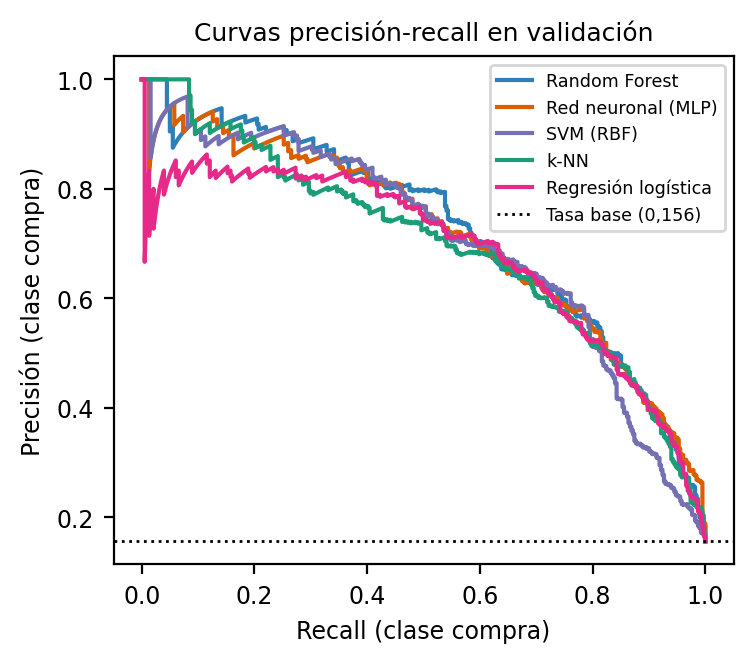
\includegraphics[width=\linewidth]{figuras/fig05_curvas_pr.png}
\centerline{(a)}
\end{minipage}\hfill
\begin{minipage}[t]{0.49\textwidth}
\centering
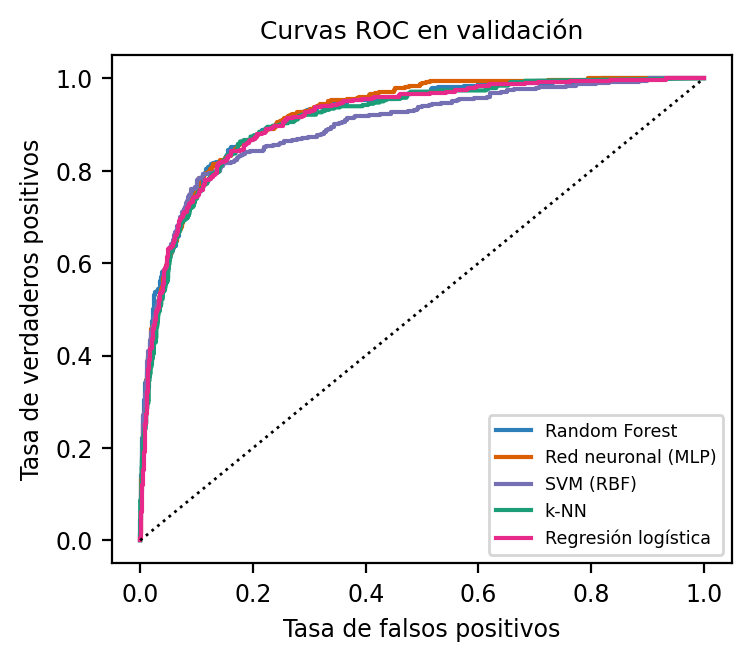
\includegraphics[width=\linewidth]{figuras/fig06_curvas_roc.png}
\centerline{(b)}
\end{minipage}
\caption{Curvas en validación. (a) Precisión-recall; la línea punteada es la tasa base
(0,156). (b) ROC; la diagonal representa un clasificador aleatorio.}
\label{fig:curvas}
\end{figure*}

La Fig.~\ref{fig:curvas} muestra las curvas precisión-recall y ROC en validación. Las
curvas de Random Forest y la MLP se cruzan en la zona de alto recall, lo que explica
que sus AP sean cercanos; la MLP conserva una ventaja pequeña en ROC-AUC porque ordena
mejor las sesiones en la zona de baja tasa de falsos positivos. Los intervalos de la
Tabla~\ref{tab:desempeno} se superponen tanto en validación como en prueba, mientras
que la regresión logística queda por debajo de forma más clara.

\begin{figure*}[t]
\centering
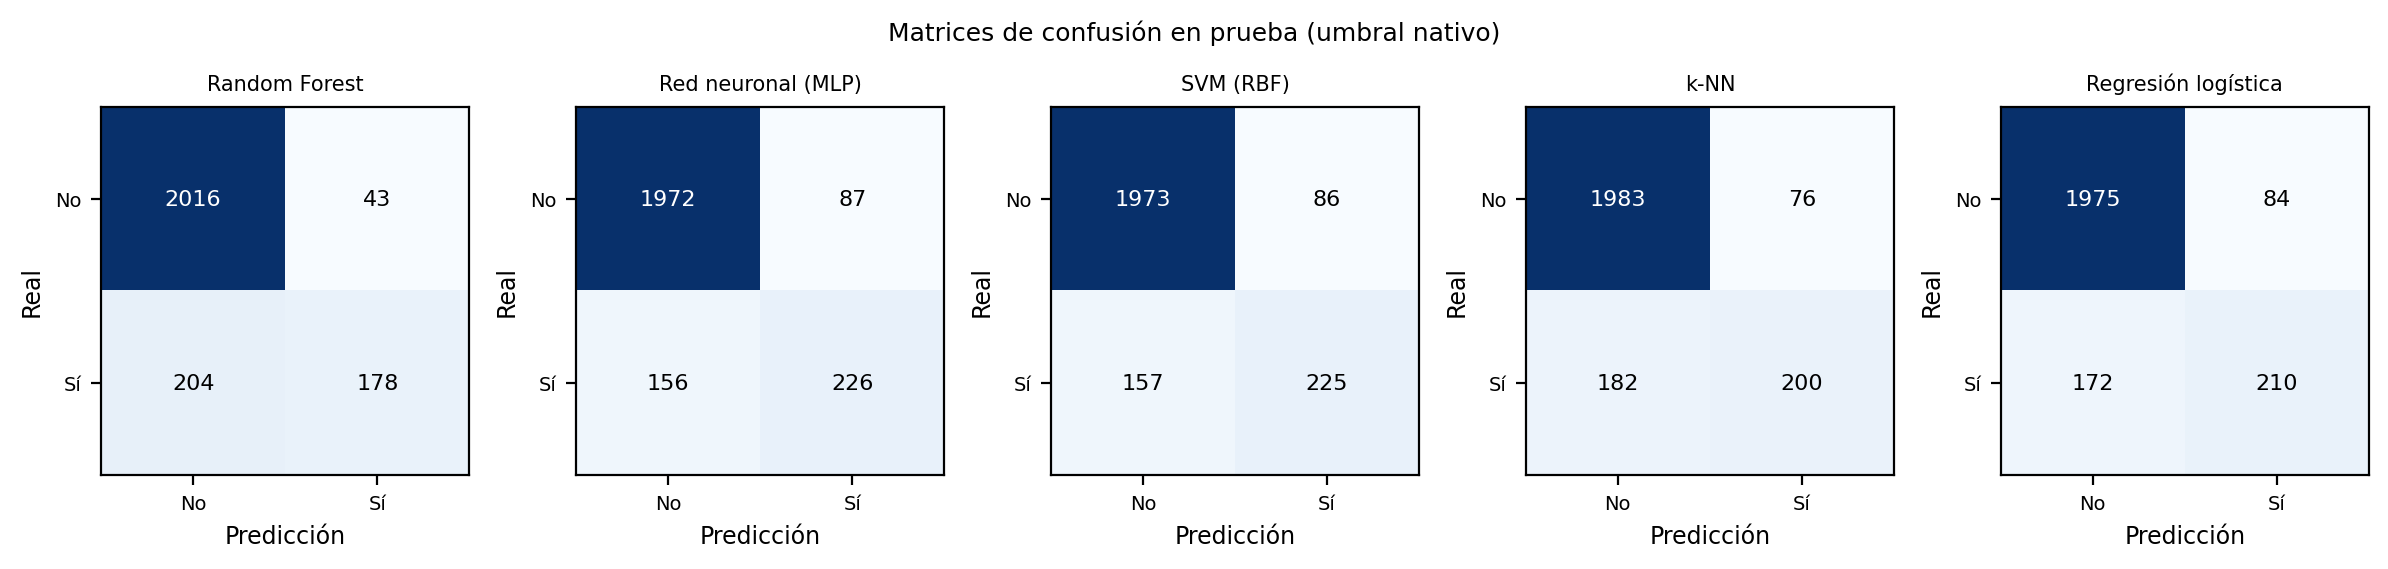
\includegraphics[width=\textwidth]{figuras/fig07_matrices_confusion_test.png}
\caption{Matrices de confusión en prueba con el umbral nativo. Las filas son la clase
real y las columnas la predicción; ``No'' es sin compra y ``Sí'' es compra.}
\label{fig:confusion}
\end{figure*}

La Fig.~\ref{fig:confusion} presenta las matrices de confusión con el umbral nativo.
Random Forest privilegia la precisión: acierta 2\,016 de 2\,059 sesiones sin compra y
178 de 382 compras, con 204 falsos negativos y 43 falsos positivos. La MLP acierta 226
compras y 1\,972 sesiones sin compra, con 156 falsos negativos y 87 falsos positivos.
SVM acierta 225 compras y 1\,973 sesiones sin compra. El perfil de Random Forest es
más conservador; el de la MLP y SVM recupera más compras a costa de más falsos
positivos. La elección depende del costo relativo de cada error.

\subsection{Umbral de decisión}

El umbral nativo de 0,5 (o 0 en la función de decisión de SVM) no es necesariamente el
mejor para una clase minoritaria. La Tabla~\ref{tab:umbral} compara el F1 con el umbral
nativo y con un umbral elegido en validación para maximizar F1. El umbral se selecciona
con la curva precisión-recall de validación y se aplica una sola vez a prueba.

\begin{table*}[t]
\centering
\caption{Efecto del umbral elegido en validación por F1 máximo. Las métricas se miden
en prueba. En SVM el umbral se aplica a la función de decisión, no a una probabilidad.}
\label{tab:umbral}
\scriptsize
\renewcommand{\arraystretch}{1.08}
\begin{tabular}{p{3.0cm} p{2.2cm} p{2.2cm} p{2.4cm} p{2.4cm} p{2.4cm}}
\toprule
\textbf{Modelo} & \textbf{Umbral} & \textbf{F1 nativo} & \textbf{F1 ajustado} & \textbf{Recall ajustado} & \textbf{Precisión ajustada} \\
\midrule
Random Forest & 0,3078 & 0,5904 & 0,6691 & 0,7173 & 0,6270 \\
MLP & 0,2230 & 0,6504 & 0,6735 & 0,7775 & 0,5940 \\
SVM & $-0{,}8475$ & 0,6494 & 0,6713 & 0,7592 & 0,6017 \\
k-NN & 0,3498 & 0,6079 & 0,6465 & 0,6728 & 0,6223 \\
Regresión logística & 0,3172 & 0,6213 & 0,6600 & 0,6885 & 0,6337 \\
\bottomrule
\end{tabular}
\end{table*}

El umbral ajustado mejora el F1 de todos los modelos y aumenta el recall de la clase
positiva. En Random Forest, el F1 pasa de 0,5904 a 0,6691 y el recall de 0,466 a
0,717; en la MLP, el F1 pasa de 0,6504 a 0,6735 y el recall de 0,592 a 0,778. El
costo es una caída de precisión: Random Forest baja de 0,805 a 0,627 y la MLP de 0,722
a 0,594. El umbral no debe fijarse solo por F1: si el costo de un falso positivo es
alto, conviene un umbral más conservador; si el costo de perder una compra es alto,
conviene el umbral ajustado. El informe reporta ambos para que la decisión sea
explícita.

\subsection{Sensibilidad y ablaciones}
\label{sec:sensibilidad}

\textit{PageValues} es la variable más influyente. La Tabla~\ref{tab:pagevalues}
compara el AP de validación con y sin ella, reajustando la malla de cada familia en el
escenario sin la variable. Al retirarla, el AP cae entre 0,34 y 0,39 en todas las
familias: Random Forest pasa de 0,7247 a 0,3852, la MLP de 0,7134 a 0,3273, SVM de
0,7049 a 0,3403, k-NN de 0,6966 a 0,3411 y la regresión logística de 0,6841 a 0,3345.
El ROC-AUC sin \textit{PageValues} también cae, pero se mantiene entre 0,756 y 0,785,
lo que indica que las demás variables conservan capacidad de ordenamiento. La
conclusión es que \textit{PageValues} domina el desempeño y que cualquier uso
operativo antes del cierre de la sesión debe asumir una pérdida grande de AP.

\begin{table}[t]
\centering
\caption{Sensibilidad al retirar \textit{PageValues}. AP de validación con y sin la
variable, y ROC-AUC sin ella.}
\label{tab:pagevalues}
\scriptsize
\renewcommand{\arraystretch}{1.08}
\setlength{\tabcolsep}{2pt}
\begin{tabular}{p{2.6cm} p{1.5cm} p{1.5cm} p{1.0cm} p{1.5cm}}
\toprule
\textbf{Modelo} & \makecell{\textbf{AP con}\\\textbf{PV}} & \makecell{\textbf{AP sin}\\\textbf{PV}} & $\Delta$\textbf{AP} & \makecell{\textbf{ROC-AUC}\\\textbf{sin}} \\
\midrule
Random Forest & 0,7247 & 0,3852 & 0,3395 & 0,7845 \\
MLP & 0,7134 & 0,3273 & 0,3861 & 0,7582 \\
SVM & 0,7049 & 0,3403 & 0,3646 & 0,7685 \\
k-NN & 0,6966 & 0,3411 & 0,3555 & 0,7564 \\
Regresión logística & 0,6841 & 0,3345 & 0,3496 & 0,7616 \\
\bottomrule
\end{tabular}
\end{table}

La ablación de \textit{SpecialDay} muestra el efecto contrario: retirarla no cambia el
AP de forma apreciable. Los cambios son $-0{,}0003$ en Random Forest, $-0{,}0030$ en
la MLP, $+0{,}0016$ en SVM, $-0{,}0059$ en k-NN y $-0{,}0004$ en la regresión
logística; los valores cercanos a cero y algunos negativos indican que el AP sin la
variable es ligeramente mayor. Esto es consistente con la equivalencia algebraica entre
el tratamiento numérico y el ordinal: como los seis niveles son equiespaciados, la
estandarización produce la misma matriz de diseño y la variable no aporta información
adicional a la que ya contienen el mes, las tasas y el resto de atributos.

\section{Análisis individual y reducción de dimensión}
\label{sec:reduccion}

Esta sección cubre el 20\,\% restante del Entregable II. Primero se evalúa cada atributo
por separado para identificar señal, redundancia y variables prescindibles. Después se
aplican PCA y UMAP sobre la matriz preprocesada y se comparan Random Forest y la MLP con
la línea base de la Sección~\ref{sec:resultados}. Todo el análisis se ajusta con el
60\,\% de entrenamiento y se evalúa en validación y prueba; la reducción se encapsula en
el \texttt{Pipeline}, de modo que PCA y UMAP se aprenden solo con entrenamiento. Tras el
one-hot y la estandarización, la matriz de diseño tiene 73 columnas.

\subsection{Análisis individual de variables}

Para cada variable numérica se calculó la correlación punto-biserial con
\textit{Revenue} y un AUC univariado, que mide hasta qué punto el atributo ordena las
sesiones por compra; para las categóricas se usó la V de Cramér y un AUC obtenido con
una regresión logística sobre su codificación one-hot. En ambos casos se añadió la
información mutua con la etiqueta. La Tabla~\ref{tab:variables-individuales} ordena las
17 variables por AUC. El AUC de las categóricas es optimista porque la regresión se
ajusta y se evalúa con los mismos datos de entrenamiento; por eso la lectura se apoya
también en la V de Cramér y en la información mutua, que son medidas descriptivas.

\begin{table*}[t]
\centering
\caption{Análisis individual de las 17 variables en entrenamiento. AUC es el área bajo
la curva ROC univariada; las variables numéricas reportan $r$ (correlación
punto-biserial) y las categóricas $V$ (V de Cramér); IM es la información mutua.
``Eliminar'' significa eliminar o combinar.}
\label{tab:variables-individuales}
\scriptsize
\renewcommand{\arraystretch}{1.02}
\setlength{\tabcolsep}{2.2pt}
\begin{minipage}[t]{0.49\textwidth}
\centering
\begin{tabular}{@{}r p{2.45cm} r r r l@{}}
\toprule
\textbf{\#} & \textbf{Variable} & \textbf{AUC} & \textbf{$r$/$V$} & \textbf{IM} & \textbf{Decisión} \\
\midrule
1 & \texttt{PageValues} & 0,866 & 0,489 & 0,165 & Mantener \\
2 & \texttt{ExitRates} & 0,710 & $-0,210$ & 0,043 & Mantener \\
3 & \texttt{ProductRelated\_}\allowbreak\texttt{Duration} & 0,669 & 0,142 & 0,032 & Mantener \\
4 & \texttt{ProductRelated} & 0,658 & 0,156 & 0,030 & Mantener \\
5 & \texttt{TrafficType} & 0,634 & 0,177 & 0,016 & Mantener \\
6 & \texttt{Administrative} & 0,626 & 0,133 & 0,016 & Mantener \\
7 & \texttt{Month} & 0,625 & 0,172 & 0,015 & Mantener \\
8 & \texttt{Administrative\_}\allowbreak\texttt{Duration} & 0,620 & 0,076 & 0,014 & Mantener \\
9 & \texttt{BounceRates} & 0,612 & $-0,148$ & 0,027 & Mantener \\
\bottomrule
\end{tabular}
\end{minipage}\hfill
\begin{minipage}[t]{0.49\textwidth}
\centering
\begin{tabular}{@{}r p{2.45cm} r r r l@{}}
\toprule
\textbf{\#} & \textbf{Variable} & \textbf{AUC} & \textbf{$r$/$V$} & \textbf{IM} & \textbf{Decisión} \\
\midrule
10 & \texttt{Informational} & 0,558 & 0,090 & 0,007 & Revisar \\
11 & \texttt{Informational\_}\allowbreak\texttt{Duration} & 0,556 & 0,066 & 0,005 & Revisar \\
12 & \texttt{OperatingSystems} & 0,555 & 0,082 & 0,004 & Revisar \\
13 & \texttt{VisitorType} & 0,546 & 0,095 & 0,004 & Eliminar \\
14 & \texttt{SpecialDay} & 0,539 & $-0,091$ & 0,009 & Eliminar \\
15 & \texttt{Browser} & 0,527 & 0,065 & 0,002 & Eliminar \\
16 & \texttt{Region} & 0,527 & 0,035 & 0,001 & Eliminar \\
17 & \texttt{Weekend} & 0,513 & 0,022 & 0,000 & Eliminar \\
\bottomrule
\end{tabular}
\end{minipage}
\end{table*}

\textit{PageValues} lidera con claridad (AUC 0,866; IM 0,165), lo que coincide con la
ablación de la Sección~\ref{sec:sensibilidad}. Le siguen \textit{ExitRates} (0,710), con
dirección negativa, y las variables de producto (0,669 y 0,658). \textit{TrafficType} y
\textit{Month} conservan señal pese a ser categóricas (0,634 y 0,625). Nueve variables
superan 0,60 y se mantienen; tres quedan entre 0,55 y 0,60 y se marcan para revisión;
cinco no superan 0,55 y son candidatas a eliminar o combinar. \textit{Weekend} es casi
indistinguible de una asignación aleatoria (0,513).

El análisis de redundancia encontró dos pares con $|r|>0{,}8$:
\textit{ProductRelated} y \textit{ProductRelated\_Duration} (0,843), y
\textit{BounceRates} y \textit{ExitRates} (0,899). Son pares casi duplicados: en un
modelo lineal conviene conservar uno de cada par, mientras que en Random Forest la
redundancia no penaliza el AP y reparte la importancia entre ambos. La decisión de
mantener todas las variables en el experimento principal es deliberada: seleccionar
variables con la etiqueta antes de particionar introduciría fuga. El análisis individual
es descriptivo y sirve para interpretar los modelos, no como paso de selección.

\subsection{Componentes principales}

PCA se ajustó dentro del \texttt{Pipeline}, después del preprocesamiento y solo con
entrenamiento, con el número de componentes elegido para retener el 95\,\% de la
varianza. Se obtuvieron 28 componentes (61,64\,\% menos columnas); el primero concentra
31,09\,\% de la varianza, los dos primeros 43,47\,\% y los cinco primeros 65,64\,\%. La
Fig.~\ref{fig:reduccion}(a) muestra la curva acumulada y el corte en 28.

\begin{figure*}[t]
\centering
\begin{minipage}[t]{0.49\textwidth}
\centering
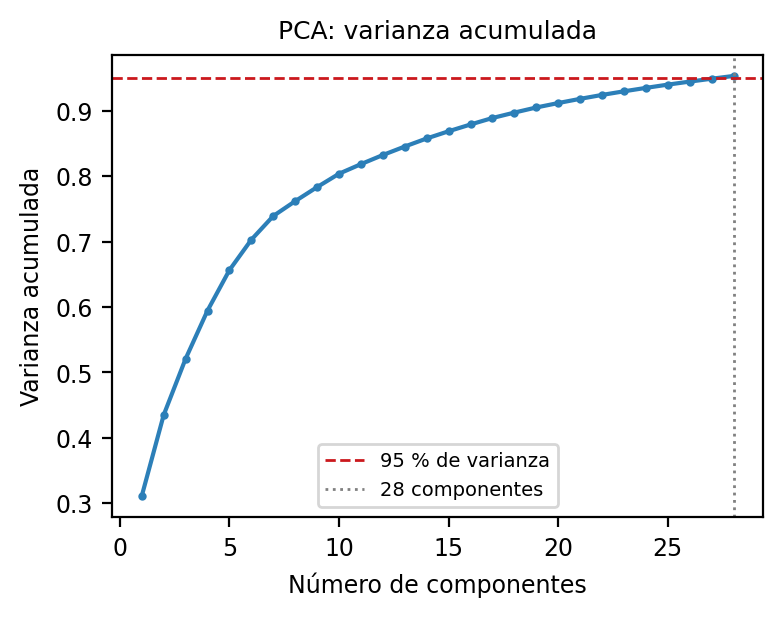
\includegraphics[width=\linewidth]{figuras/fig11_pca_varianza.png}
\centerline{(a)}
\end{minipage}\hfill
\begin{minipage}[t]{0.49\textwidth}
\centering
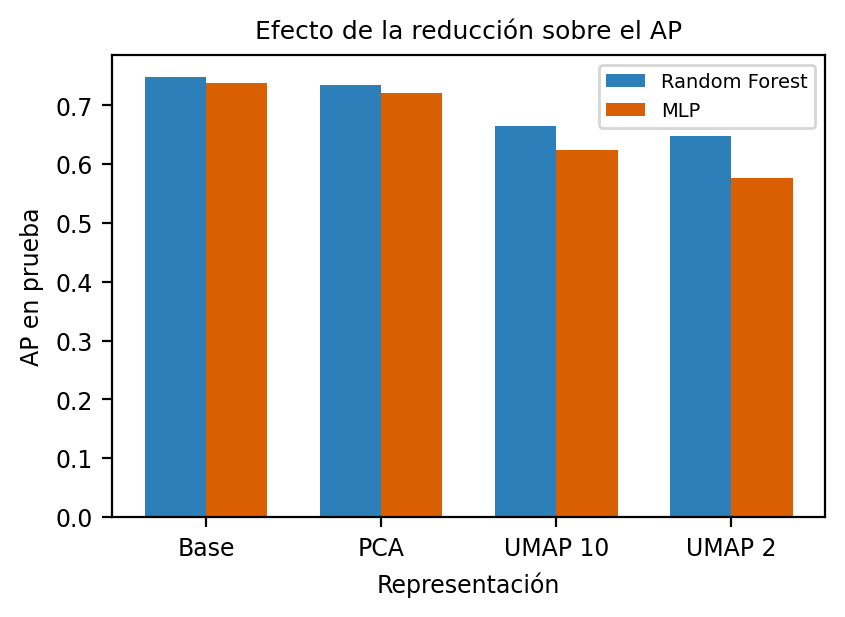
\includegraphics[width=\linewidth]{figuras/fig13_comparacion_reduccion.png}
\centerline{(b)}
\end{minipage}
\caption{Reducción de dimensión. (a) Varianza acumulada de PCA; el corte retiene 28
componentes para el 95\,\%. (b) AP de prueba con la representación original, PCA, UMAP
de 10 componentes y UMAP de 2.}
\label{fig:reduccion}
\end{figure*}

La Tabla~\ref{tab:reduccion} compara el AP de prueba. Con PCA, Random Forest pasa de
0,7486 a 0,7352 ($\Delta=-0{,}0134$) y la MLP de 0,7377 a 0,7211 ($\Delta=-0{,}0165$);
el ROC-AUC se mantiene por encima de 0,92 en ambos casos y el F1 de Random Forest sube
de 0,5904 a 0,6254 porque la representación cambia la distribución de scores y el umbral
nativo. La pérdida de AP es pequeña frente a la reducción de 61,6\,\% de las columnas:
PCA conserva la estructura lineal que separa las compras. En validación, la MLP con PCA
incluso mejora su AP (0,7189 frente a 0,7134), aunque la ventaja no se repite en prueba;
esa discrepancia recuerda que la validación tiene 2\,441 sesiones y una sola partición.

\subsection{Proyección UMAP}

UMAP se ajustó con 10 componentes, 15 vecinos y \textit{min\_dist}=0,1, también dentro
del \texttt{Pipeline}; se eligieron 10 como compromiso entre reducción y señal, y 2 solo
para la visualización. La reducción es del 86,30\,\% (10 columnas frente a 73). El AP de
prueba cae a 0,6650 en Random Forest ($\Delta=-0{,}0836$) y a 0,6236 en la MLP
($\Delta=-0{,}1141$); el ROC-AUC baja a 0,8923 y 0,8571. La caída es mucho mayor que la
de PCA y crece al reducir a dos dimensiones: UMAP2 deja el AP en 0,6489 y 0,5762,
respectivamente. La Fig.~\ref{fig:umap} muestra la proyección 2D en prueba: las clases
se superponen y no forman dos grupos separados; la tasa de compra aumenta con la segunda
coordenada, lo que explica que UMAP2 conserve algo de señal pero pierda AP. UMAP
preserva vecindades locales, pero no la dirección lineal que separa las compras; además
es estocástico y más costoso (48,1 s para Random Forest frente a 7,0 s con PCA).

\begin{figure}[t]
\centering
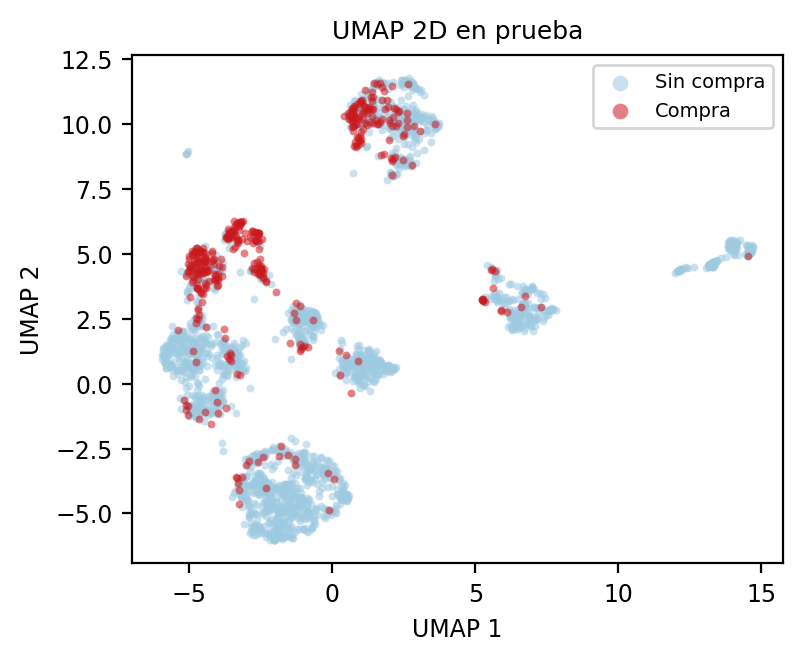
\includegraphics[width=\columnwidth]{figuras/fig12_umap_2d.png}
\caption{Proyección UMAP en dos dimensiones del conjunto de prueba. Cada punto es una
sesión; el color indica si terminó en compra.}
\label{fig:umap}
\end{figure}

\begin{table}[t]
\centering
\caption{Efecto de la reducción sobre el AP de prueba. $\Delta$ se mide frente a la
línea base con las 73 columnas.}
\label{tab:reduccion}
\scriptsize
\renewcommand{\arraystretch}{1.05}
\setlength{\tabcolsep}{2pt}
\begin{tabular}{@{}l r r r r r r@{}}
\toprule
\textbf{Repr.} & \textbf{Comp.} & \textbf{Red.} & \textbf{AP RF} & \textbf{$\Delta$ RF} & \textbf{AP MLP} & \textbf{$\Delta$ MLP} \\
\midrule
Base & 73 & 0\,\% & 0,7486 & --- & 0,7377 & --- \\
PCA & 28 & 61,6\,\% & 0,7352 & $-0{,}0134$ & 0,7211 & $-0{,}0165$ \\
UMAP10 & 10 & 86,3\,\% & 0,6650 & $-0{,}0836$ & 0,6236 & $-0{,}1141$ \\
UMAP2 & 2 & 97,3\,\% & 0,6489 & $-0{,}0996$ & 0,5762 & $-0{,}1615$ \\
\bottomrule
\end{tabular}
\end{table}

La comparación deja una conclusión práctica: PCA es la única reducción que conserva el
desempeño; UMAP degrada el AP entre 8 y 16 puntos y no compensa el ahorro de columnas.
Para este conjunto, con 73 columnas y 7\,323 sesiones de entrenamiento, el costo de
mantener las variables originales es menor que la pérdida de señal. La reducción tendría
sentido si el objetivo fuera desplegar el modelo con menos memoria o visualizar los
perfiles, no si el objetivo es maximizar el AP. El análisis individual y la reducción
completan así el diagnóstico de la Sección~\ref{sec:resultados}: la señal se conserva en
28 direcciones y se pierde cuando UMAP prioriza vecindades locales.

\section{Discusión y conclusiones}
\label{sec:conclusiones}

El diseño experimental permitió comparar cinco familias de modelos bajo un protocolo
común, con el preprocesamiento y la selección de transformaciones ajustados
exclusivamente dentro de los folds y con un conjunto de prueba aislado. Random Forest
obtuvo el mayor AP en validación y prueba, con 0,7247 y 0,7486, respectivamente. La MLP
quedó segunda en AP (0,7134 y 0,7377) y primera en ROC-AUC de prueba (0,9270 frente a
0,9242). Las comparaciones pareadas muestran que la diferencia en AP
($+0{,}0104$, IC $[-0{,}0100;0{,}0321]$) y la diferencia en ROC-AUC
($-0{,}0029$, IC $[-0{,}0101;0{,}0040]$) no son significativas. Por lo tanto, Random
Forest y la MLP son estadísticamente equivalentes; la elección entre ambos debe
hacerse por criterios operativos: interpretabilidad, costo de cómputo, calibración y
perfil de errores.

El umbral de decisión es una decisión de negocio, no un detalle técnico. Con el umbral
nativo, Random Forest privilegia la precisión y deja escapar más de la mitad de las
compras (recall 0,466). Con el umbral ajustado por F1 en validación, el recall sube a
0,717 y el F1 a 0,6691, a costa de bajar la precisión a 0,627. La MLP y SVM ofrecen un
perfil intermedio. Se reportan ambos umbrales para hacer explícito ese compromiso.

\textit{PageValues} es la variable dominante: su AUC univariado es 0,866 y retirarla
reduce el AP entre 0,34 y 0,39, muy por encima del efecto de cualquier hiperparámetro.
\textit{ExitRates} y las variables de producto le siguen, mientras que \textit{Weekend},
\textit{Region}, \textit{Browser}, \textit{VisitorType} y \textit{SpecialDay} aportan
poco. Esto delimita el alcance: el modelo sirve para analizar sesiones cerradas y
priorizar acciones posteriores, no para decidir durante la sesión. Un sistema en tiempo
real tendría que operar sin \textit{PageValues} y asumir la pérdida de AP documentada en
la Tabla~\ref{tab:pagevalues}.

La reducción de dimensión confirma que la señal está concentrada. PCA retuvo 28
componentes (95,34\,\% de la varianza y 61,64\,\% menos columnas) y conservó el AP
dentro de 1,7 puntos; UMAP, en cambio, lo degradó entre 8 y 16 puntos. Para este tamaño
de datos, reducir con PCA es razonable; UMAP sirve para visualizar, no para modelar.

El trabajo tiene limitaciones. Usa una sola base de datos y una sola semilla, con
particiones estratificadas pero no temporales, de modo que no evalúa la deriva entre
periodos. No calibró probabilidades ni hizo un análisis formal de costo-beneficio; el
umbral se eligió por F1. La clase positiva tiene 1\,908 casos, lo que limita la
precisión de los intervalos, y UMAP añade variabilidad por su inicialización aleatoria.
Como trabajo futuro se propone validación temporal, calibración, umbrales sensibles al
costo y repetir el experimento con otras semillas.

En síntesis, el protocolo evita fugas, reporta incertidumbre y distingue ranking de
decisión. Random Forest y la MLP son los finalistas, sin diferencia estadística;
\textit{PageValues} explica la mayor parte del desempeño y el umbral ajustado mejora el
recall a cambio de precisión. PCA conserva la señal en 28 direcciones; UMAP no la
preserva.

\begin{thebibliography}{5}

\bibitem{ref_dataset}
C.~Sakar and Y.~Kastro, ``Online Shoppers Purchasing Intention Dataset,'' UCI Machine
Learning Repository, 2018. [Dataset]. doi: 10.24432/C5F88Q. [Online]. Available:
\url{https://doi.org/10.24432/C5F88Q}

\bibitem{ref_sakar}
C.~O.~Sakar, S.~O.~Polat, M.~Katircioglu, and Y.~Kastro, ``Real-time prediction of
online shoppers' purchasing intention using multilayer perceptron and LSTM recurrent
neural networks,'' \textit{Neural Computing and Applications}, vol.~31, no.~10,
pp.~6893--6908, 2019. doi: 10.1007/s00521-018-3523-0.

\bibitem{ref_necula}
S.-C.~Necula, ``Exploring the impact of time spent reading product information on
e-commerce websites: A machine learning approach to analyze consumer behavior,''
\textit{Behavioral Sciences}, vol.~13, no.~6, Art.~no.~439, 2023.
doi: 10.3390/bs13060439.

\bibitem{ref_satu}
M.~S.~Satu and S.~F.~Islam, ``Modeling online customer purchase intention behavior
applying different feature engineering and classification techniques,''
\textit{Discover Artificial Intelligence}, vol.~3, Art.~no.~36, 2023.
doi: 10.1007/s44163-023-00086-0.

\bibitem{ref_lin}
J.~Lin, ``Application of machine learning in predicting consumer behavior and
precision marketing,'' \textit{PLOS ONE}, vol.~20, no.~5, Art.~no.~e0321854, 2025.
doi: 10.1371/journal.pone.0321854.

\end{thebibliography}

\end{document}
